\section{Evaluation}
To evaluate our design and implementation, we compare the performance of the modified \textit{AC-BPFS} on a storage hierarchy of NVM and disk with that of the original \textit{BPFS}~\cite{c10} on NVM and \textit{ext4} (ordered mode) on disk. We use the performance of the original \textit{BPFS} on NVM as a baseline and focus on the following key questions:

\begin{itemize}
\item What is the overhead of the anti-caching mechanisms implemented on top of \textit{BPFS}? \vspace{-0.1in}
\item What is the performance of \textit{AC-BPFS} in the presence of eviction of cold blocks? \vspace{-0.1in}
\item How does performance of \textit{AC-BPFS} differ for various anti-caching eviction thresholds? \vspace{-0.1in}
\item How does the degree of hotness and coldness of stored data affect the performance of the system? \vspace{-0.1in}
\end{itemize}

\textbf{Hypotheses:} Our hypothesis is that when accessing hot data on NVM, \textit{AC-BPFS} should perform similar to \textit{BPFS}. If our design is right, eviction of cold data blocks by anti-cache manager in the background should not affect the performance of \textit{AC-BPFS}. Cold data block access latency will be similar to that of \textit{ext4} and this cost of accessing cold data on disk will be amortized in the presence of hot data accesses in the workloads. We run various micro-benchmarks and filebench~\cite{filebench} macro-benchmark to evaluate if these hypotheses are true.

\subsection{Methodology and Setup}
Making a meaningful performance comparison of \textit{AC-BPFS} with both NVM file system such as \textit{BPFS} and disk based file system such as \textit{ext4}, presents challenges at different levels. We cannot make a comparison in isolation since our implementation is a hybrid approach that incorporates both NVM and disk. Since \textit{ext4} filesystem buffers writes in operating system buffer cache, we issue \textit{fsync} in our workloads so that the data is made durable on disk. This makes our comparison reasonable as issuing \textit{sync} on \textit{AC-BPFS} and \textit{BPFS} flushes the CPU caches making the data durable on NVM. 

For the purpose of the evaluation, we run our experiments on a real hardware with 8 CPU cores running Ubuntu linux operating system with 16 GB of main memory, 1 TB of hard disk drive. We simulate the behavior of NVM using DRAM due to unavailability of the hardware. Unless otherwise noted, both the original and our implementation of \textit{BPFS} are mounted in 2GB of main memory. The anti-caching daemon is set to run at 10 ms by default with anti-caching threshold of 40 MB for micro-benchmarks while varying the anti-caching threshold for the macro-benchmark.

\subsection{Micro-benchmarks}
In this section we present an experimental evaluation of \textit{AC-BPFS} on NVM and disk using a set of micro-benchmarks and offer comparisons with those of \textit{BPFS} on NVM and \textit{ext4} on disk. 

\subsubsection{Micro-benchmark: Various Filesystem Operations}
In order to ensure the correctness of various filesystem operations and to measure if there is any additional overhead due to anti-caching mechanisms implemented on top of \textit{BPFS}, we benchmarked different file operations in \textit{AC-BPFS} and compare the performance with that of \textit{BPFS}. Table~\ref{tbl-micro} shows a representative sample of those operations and latency for each of these operation for both \textit{AC-BPFS} and \textit{BPFS}. We benchmark \textit{read}, \textit{write} and \textit{append} operations in a later subsection. 

\newcolumntype{P}[1]{>{\centering\arraybackslash}p{#1}}
\begin{table}[!t]
%\vspace{0.1in}
\begin{center}
{\footnotesize
\begin{tabular}{c|P{2.5cm}|P{2.5cm}}
\textbf{Operations} & \textbf{AC-BPFS latency(ms)} & \textbf{BPFS latency(ms)} \\
\hline
chmod&5.26&5.19 \\
create&6.49&6.45 \\
link&6.21&6.24 \\
mkdir&6.61&6.55 \\
readdir&3.24&3.1 \\
rename\_dir&8.3&7.61 \\
rename\_file&8.6&7.82 \\
rmdir&6.66&5.95 \\
symlink&6.58&6.46 \\
unlink\_16M&10.03&10.42 \\
unlink\_hardlink&5.5&5.5 \\
\end{tabular}
}
\end{center}
\vspace{-0.1in}
\mycaption{tbl-micro}{Micro-benchmark}{\footnotesize This table shows a set of filesystem operations and latency for each of these operations in both \textit{AC-BPFS} and \textit{BPFS}
}
\end{table}

\textbf{Analysis:} The table~\ref{tbl-micro} shows that for the file operations the added overhead is negligible, if any at all thus showing that the various anti-caching mechanisms implemented on top of \textit{BPFS} do not add an additional overhead. The filesystem operations shown in table~\ref{tbl-micro} do not include operations that access cold data and involve only meta data blocks like inode and directory entries except for unlink where data blocks on disk needs to be freed if any (Note that freeing of data blocks on dis is asynchronous and happens in the background). Hence all the accesses are to NVM, the performance of \textit{AC-BPFS} and \textit{BPFS} should be similar and the data reflects this.

 \begin{figure*}[t]\centering
\begin{subfigure}{.46\textwidth}
  \centering
  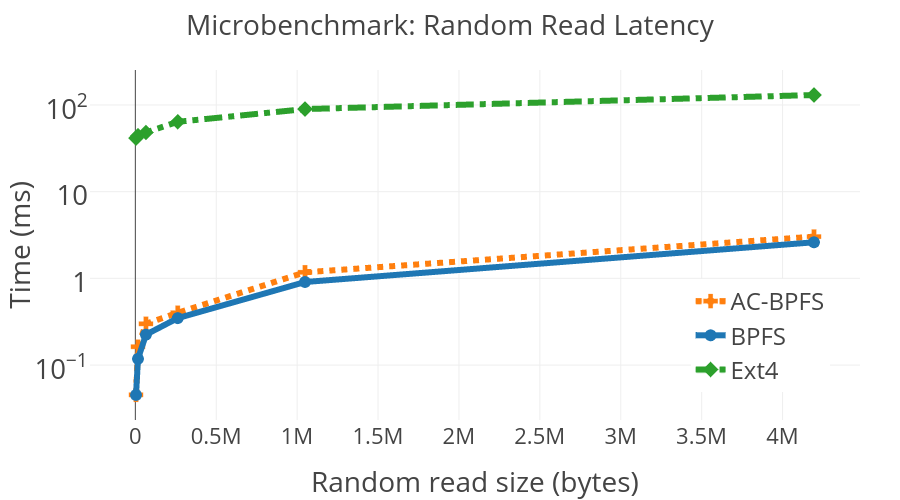
\includegraphics[width=\linewidth]{figs/read.png}
 	\centering
	\footnotesize\textit{(a) Micro-benchmark: Read}
\end{subfigure}
\begin{subfigure}{.46\textwidth}
  \centering
  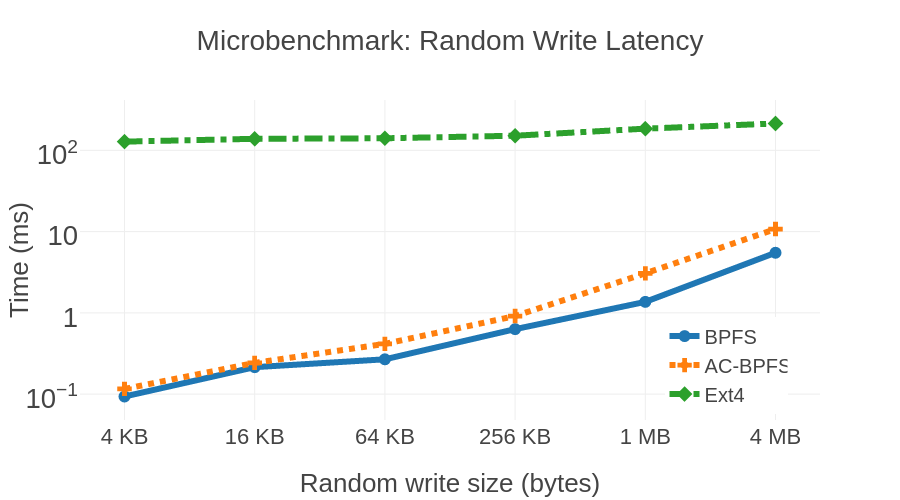
\includegraphics[width=\textwidth]{figs/write.png}
\vspace{-0.2in}
\caption{Micro-benchmark: Write}
\end{subfigure}
\caption{Micro-benchmarks}{\footnotesize The figure shows the append latency of \textit{AC-BPFS} for various sizes. The figure shows the write latency of \textit{AC-BPFS} for various sizes}
\label{fig:fig}
\end{figure*}


\begin{figure}
\centering
\vspace{-0.1in}
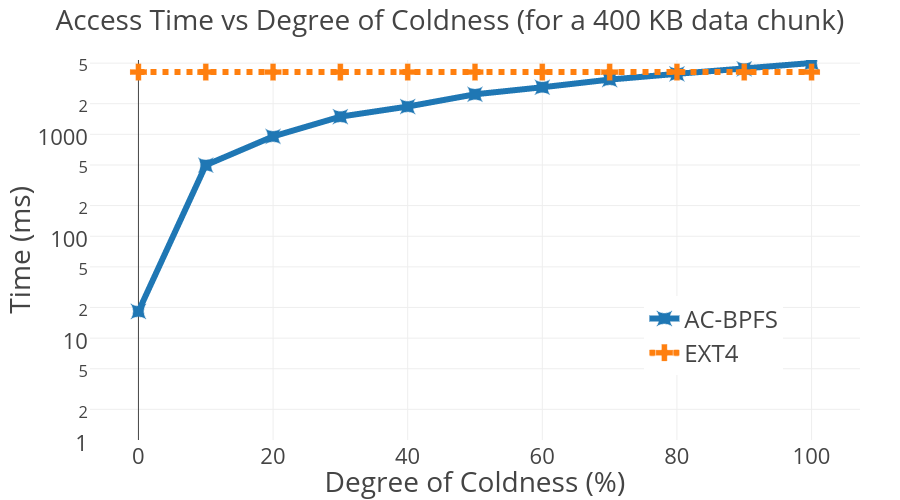
\includegraphics[width=0.5\textwidth]{figs/coldness.png}
\vspace{-0.1in}
\mycaption{fig-coldness}{Impact of Degree of Coldness on Read Latency}{\footnotesize This figure shows the block read latency for various degrees of coldness}
\end{figure}


\subsubsection{Micro-benchmark: Random write}
. We evaluated the performance of making random write operations for various data size for AC\_BPFS, \textit{BPFS} and  \textit{ext4} . For the AC\-BPFS, to ensure uniform distribution of write operations to data blocks in both the persistent memory and the disk, we pre-generated a list of files of various sizes and random offsets with in those files. We ensured that data chucks written at random offsets exceeded the pre-specified cache threshold to force seek from the disk. We called 'fsync' after every write call to force the data to disk so as to make even comparisons across the filesystems. We used UNIX 'clock\_gettime' system call to measure the time for this benchmark.

Figure~\ref{fig-write} shows the results for this micro-benchmark. Both AC\_BPFS and \textit{BPFS} are faster than the  \textit{ext4}  in orders of magnitude, as we hoped. It also shows that AC\-BFPS, although starts to lag behind the \textit{BPFS} as the size of the data being written increases, it does not lag significantly, that reinforces our initial intuition and supports our objective.



\subsubsection{Micro-benchmark: Append}
We measured the cost of appending data chunks of various size to an empty file. As with the benchmark for the random write, we called ‘fsync’ after every write call to ensure that the data gets written to the disk. We used UNIX 'clock\_gettime' system call to measure the time for this benchmark.

As with random write, Figure~\ref{fig-append}  shows that both AC\-BPFS and \textit{BPFS} are faster than the  \textit{ext4}  in orders of magnitude. Since the writing of all the data for the ‘append’ operation happened entirely in memory, AC\-BPFS and \textit{BPFS} performance lines are virtually inseparable. This result justifies the anti-caching mechanism that we have employed and also illustrates its low overhead.


\subsubsection{Micro-benchmark: Degree of coldness}
This micro-benchmark demonstrates the effect of the anti-caching and plots the read latency of reading 400 KB data against the degree of coldness. For the benchmark, we read a 400 KB chunk of data, part of which can be hot/cold depending on the degree of coldness. A 20\% coldness factor on the X-axis for a 400 KB chunk data size would mean that 80 KB of the 'cold' data resides in the disk, while 320 KB of 'hot' data resides in NVM. So as expected, the read latency for a 20\% cold data would be less than the read latency for a 80\% cold data.\\

 At a 100\% level, the performance will flat-line with the  \textit{ext4}  performance. To implement this benchmark, we create 10 files of 40 KB each and we fix our anti-cache size to be 40 KB, so that at any given point only 1 file can reside in NVM. Then a workload is created, which simulates the reading of certain number of files in the NVM vs the files in the disk, based on the degree of coldness. As it is evident Figure~\ref{fig-coldness}, at 0\% coldness our performance is exactly what you would expect from \textit{BPFS}, while at 100\% coldness it slightly overshoots the  \textit{ext4}  performance. \\

This is understandable given the overhead for us, in terms of anti-caching daemon. However, the most interesting part of this graph is that the trend as one increases the degree of coldness. The less the degree of coldness, the more is the performance. This clearly proves the benefit of our anti-caching implementation for a tiered storage.

 
\subsubsection{Macro-benchmark: File Bench}
For this benchmark, we used FileBench to test and compare the performance of the three files systems by generating a large variety of workloads {cite} of size 1.25 GB. The workload is comprised of 33\% read requests and 67\% write requests. For the AC\-BPFS, we ran the benchmark by varying the (anti) caching thresholds – from 20\% of the workload size to 100\% of the workload size. We did so in order to get insights on the effectiveness and overheads of the anti-caching mechanisms in addition to making comparison of the AC\-BPFS with \textit{BPFS} and  \textit{ext4}  file systems.


 \begin{figure*}[t]\centering

\begin{subfigure}{.49\textwidth}
\centering
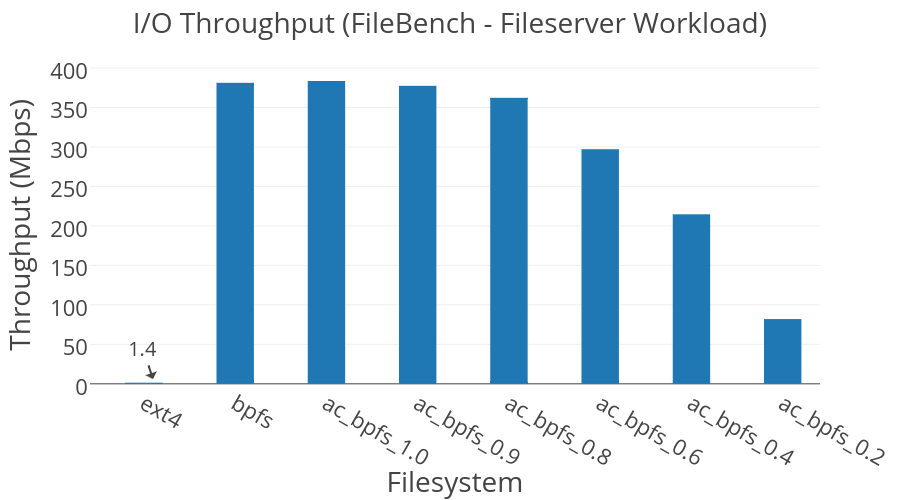
\includegraphics[width=0.9\textwidth]{figs/filebench.png}
\mycaption{fig-fb}{FileBench (FileServer) - I/O Throughput}{\footnotesize This figure shows the I/O throughput of  \textit{ext4} , \textit{BPFS} and \textit{AC-BPFS} under various configurations for the FileServer workload in FileBench}
\end{subfigure}
\begin{subfigure}{.49\textwidth}
\centering
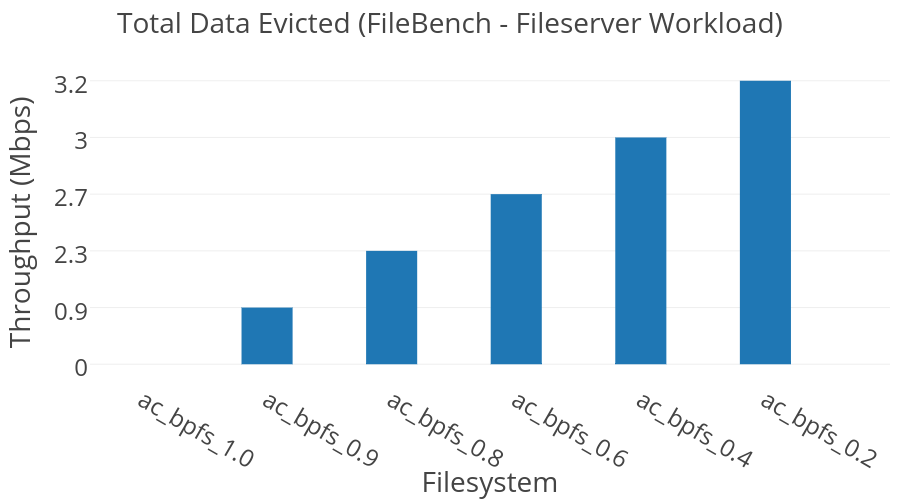
\includegraphics[width=0.9\textwidth]{figs/bench2.png}
\mycaption{fig-fb2}{FileBench (FileServer) - Block Eviction Count}{\footnotesize This figure shows the number of data blocks evicted from NVM under various configurations for the FileBench file server workload}
\end{subfigure}

\caption{Macro-benchmarks}
\label{fig1:fig1}
\end{figure*}

The Figure~\ref{fig-fb} shows that when the caching threshold is 100\% of the workload size (i.e. all the operations happen in the persistent memory), the performance of AC\-BPFS is identical to that of \textit{BPFS}, as we expected. As we decrease the caching threshold, the performance suffers accordingly. On all times, the performance of the AC\-BPFS is better than that of  \textit{ext4}  in orders of magnitude.
